\documentclass[12pt,a4paper]{report}
\usepackage[utf8]{inputenc}
\usepackage[spanish]{babel}
\usepackage{amsmath}
\usepackage{amsfonts}
\usepackage{amssymb}
\usepackage{graphicx}
\usepackage{listings}
\usepackage[usenames,dvipsnames]{color}
\usepackage[numbers,sort&compress]{natbib} 
\usepackage{natbib}
\usepackage[left=2cm,right=2cm,top=2cm,bottom=2cm]{geometry}
\author{ Paola Lizbeth Vázquez}


\title{Matemáticas Computacionales \\ Práctica 1: Gráficas de curvas en R} %Título del documento
\author{Profesor: Ángel Isabel Moreno Saucedo \\ Alumno: Paola Lizbeth Vázquez Leal \\ Semestre Febrero - Junio 2021} %Autor del documento
\date{18 de febrero de 2021}

\begin{document}

\maketitle %Para crear el título del documento
Practica 01
\section{Introducción}
En esta primera actividad podremos observar comose grafican algunas rectas y curvas en $\mathbb{R}^2$, además de recordar datos principales de estas misma, como son su definicion y formula. Las curvas a repasar y graficar son la recta, parábola, circunferencia, elipse e hipérbola.


\section{Curvas de $\mathbb{R}^2$} 

\subsection{Línea recta} \label{subsec:linearecta}

\textbf{Definición.}Es aquel lugar geométrico que se crea tomando dos puntos cualesquiera ($P_1(x_1, y_1)$, $P_2(x_2, y_2)$) del lugar.  Para calcular la pendiente de una recta tenemos 
\begin{equation}
m = \frac{y_1-y_2}{x_1-x_2} \label{eq:pendiente}
\end{equation}

Seguido de esto tenemos la ecuación general de la recta:
\begin{equation}
Ax + By + C = 0, \label{eq:recta}
\end{equation}

Donde una recta que pasa por el punto dado $P_1(x_1,y_1)$ y tiene una pendiente dada por (\ref{eq:pendiente}), tiene de ecuación

\begin{equation}
y-y_1=m(x-x_1) \label{eq:rectapend}
\end{equation}
 de la cual para poder  graficar en $\mathbb{R}^2$ se busca despejar $y$ de (\ref{eq:rectapend}).
 
\begin{equation}
y = mx + b \label{eq:pendienteinterseccion}
\end{equation}

Para graficar esta función se dan valores a $m$, $x$ y $b$, con los cuales se podrá formar una gráfica deseada. 

A continuación se tienen dos ejemplos de linea recta.


\begin{figure}
\centering
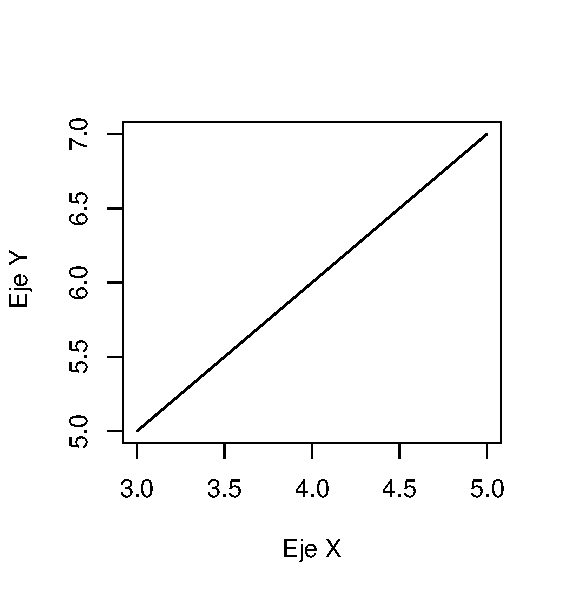
\includegraphics[scale = 0.8]{Recta1}
\caption{Grafica 1. Con pendiente m = 1.}
\label{fig:Recta1}
\end{figure}

\begin{figure}
\centering
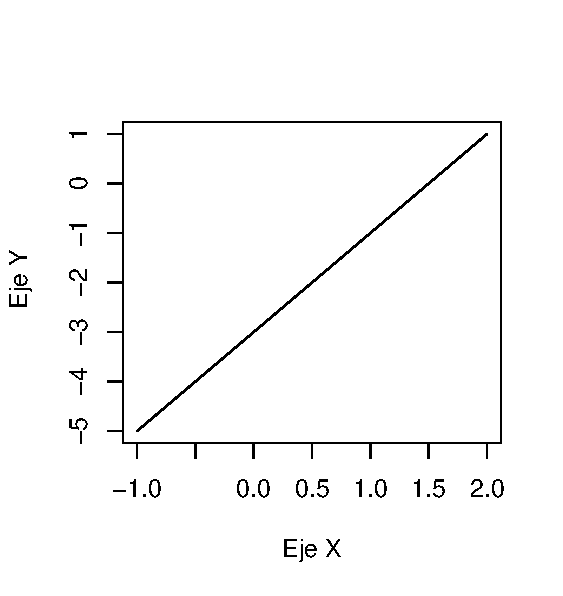
\includegraphics[scale = 0.8]{Recta2}
\caption{Grafica 2. Con pendiente m = 2.}
\label{fig:Recta2}
\end{figure}

\newpage
\subsection{La Parábola} \label{subsec:parabola}
\textbf{Definición.}La parabola se mueve en un plano de manera que la distancia de una recta fija, es siempre igual a su distancia de un punto fijo dentro del plano.
El punto fijo es conocido como $foco$  y la recta fija es llamada $directriz$ de la parábola. 


Si llamamos $F$ y $l$ al foco y directriz de una parábola, la recta $a$ que pasa por $F$ y es perpendicular a la $l$ se llama eje de la parábola.

Para gráficar la parábola se hará utilizando la ecuación (\ref{eq:parabola}), en su forma general.
\begin{equation}
y = Ax^2 + Bc + C \label{eq:parabola}
\end{equation}

Al evaluar la ecuación (\ref{eq:parabola}) en los valores dados podemos obtener principalmente los valores de la función y. Continuamente se puede obtener la gráfica de estos. 


\begin{figure}
\centering
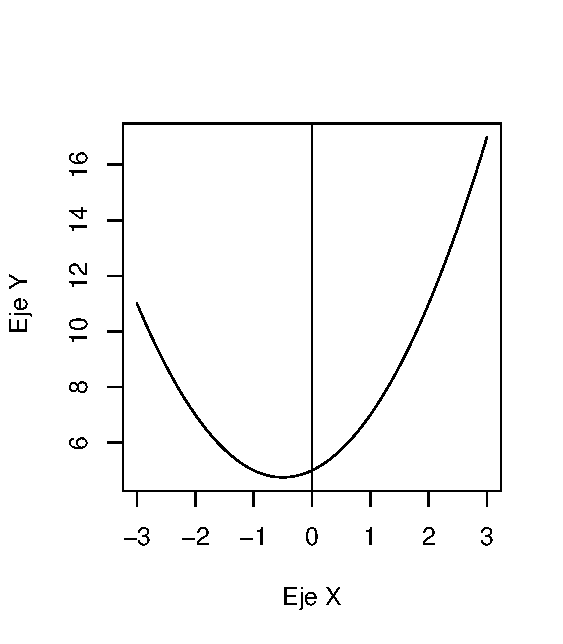
\includegraphics[scale=0.8]{Parabola1}
\caption{Gráfica 1. De la ecuación $y = x ^2 + x + 5$.}
\label{fig:Parabola1}
\end{figure}

\begin{figure}
\centering
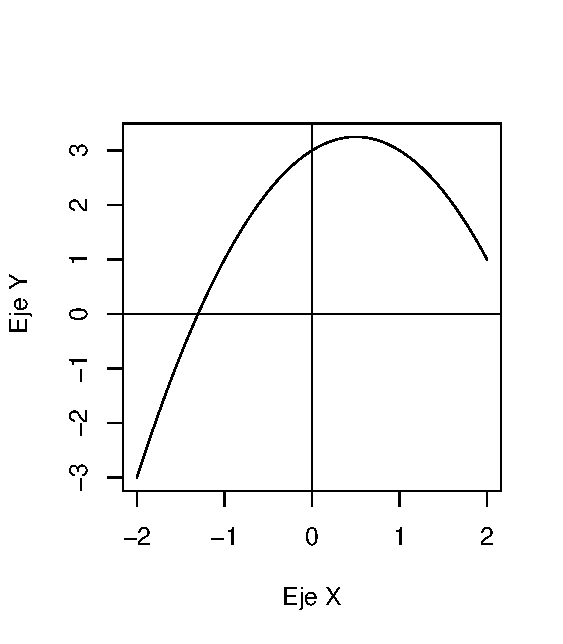
\includegraphics[scale=0.8]{Parabola2}
\caption{Gráfica 2. De la ecuación $y = -x ^2 + x + 3$.}
\label{fig:Parabola2}
\end{figure}


\newpage
\subsection{Circunferencia} \label{subsec:circunferencia}

\textbf{Definición.}Entendemos como circunferencia al lugar geométrico ubicado en un punto cualquiera. Esta contiene un punto fijo llamado centro y se mantiene siempre a una distancia del $centro$, siendo esta el $radio$. 
Siendo el centro $C(h, k)$ y el radio es la constante $r$.

Tenemos la ecuacion de la circunferencia dada por:
\begin{equation}
(x - h)^2 + (y - k)^2 = r^2, \label{eq:circunferencia}
\end{equation}

Con los datos anteriormente mencionados se podrá realizar la grafica de la circunferencia. 
Principalmente, tomando la ecuación (\ref{eq:circunferencia}), se despejará con respecto a $y$ obteniendo la siguiente ecuación.
\begin{equation}
y = k \pm \sqrt{r^2 - (x - h)^2}, \label{eq:cdespejada}
\end{equation}

Para obtener la gráfica de manera correcta se restringira el dominio en en $x \in [h - r, h + r]$. Se codificará una función que reciba todos los datos dados como entrada y entregue como salida la gráfica de la circunferencia con centro en $(h, k)$ y radio $r$.

\begin{figure}
\centering
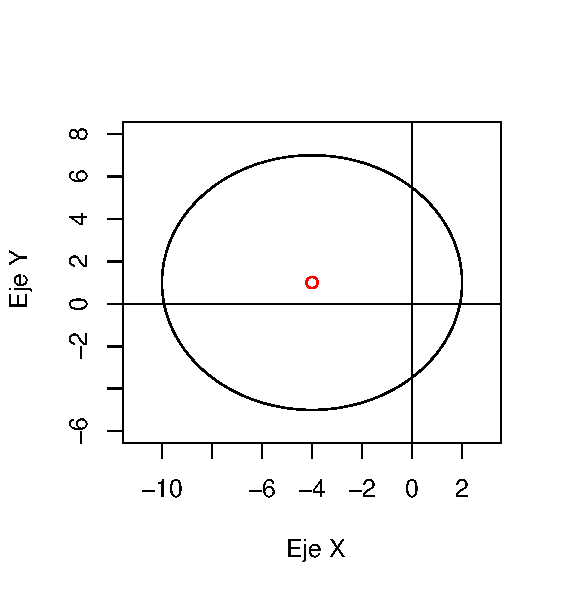
\includegraphics[scale=0.9]{Circunferencia1}
\caption{Grafica de una circunferencia con centro en (-4, 1) y radio 6.}
\label{fig:Circunferencia1}
\end{figure}

\begin{figure}
\centering
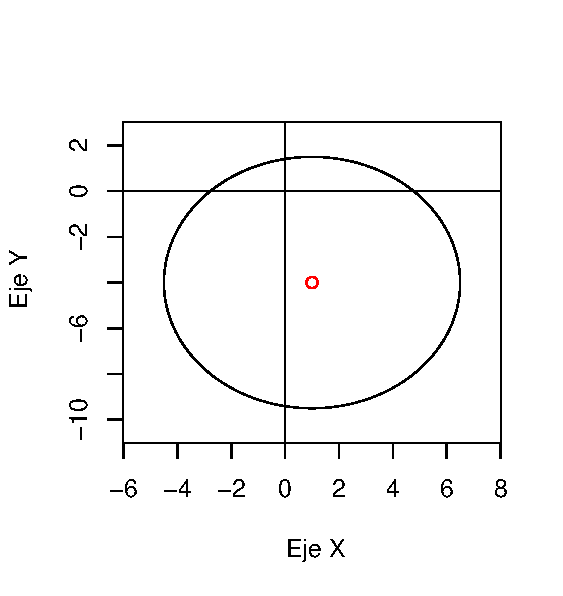
\includegraphics[scale=0.9]{Circunferencia2}
\caption{Grafica de una circunferencia con centro en (1, -4) y radio 5.5.}
\label{fig:Circunferencia2}
\end{figure}

\newpage
\subsection{Elipse}

\textbf{Definición.} Se le conoce como el lugar geométrico de un punto que se mueve en un plano de manera que la suma de sus distancias a dos puntos fijos de ese plano es siempre igual a una constante mayor que la distancia etre los dos puntos.

Los puntos fijos son llamados $focos$ de la elipse. 


Para graficar una elipse  se tiene principalmente la ecuación ordinaria:


\begin{equation}
\frac{(y-k)^2}{a^2}+  \frac{(x-h)^2}{b^2}= 1 \label{eq:elipse}
\end{equation}

 de (\ref{eq:elipse}) se despejará la variable $y$.
 
\begin{equation}
y = k \pm \sqrt{b^2 - \frac{b^2}{a^2}(x - h)^2} \label{eq:elipsedes}
\end{equation}

con un dominio $x \in [h - a, h + a]$ ó $x \in [h - b, h + b]$ según el caso. 

\begin{figure}
\centering
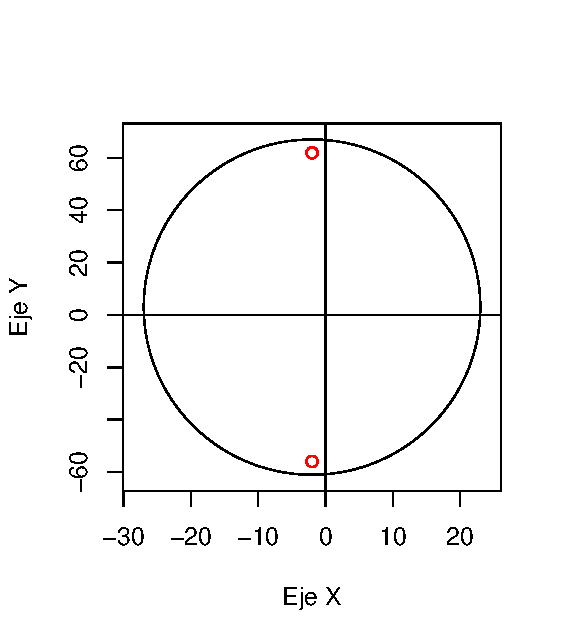
\includegraphics[scale=0.9]{Elipse1}
\caption{Gráfica de una elipse horizontal con centro en (-2, 3), $a = 64$ y $b = 25$.}
\label{fig:Elipse1}
\end{figure}

\begin{figure}
\centering
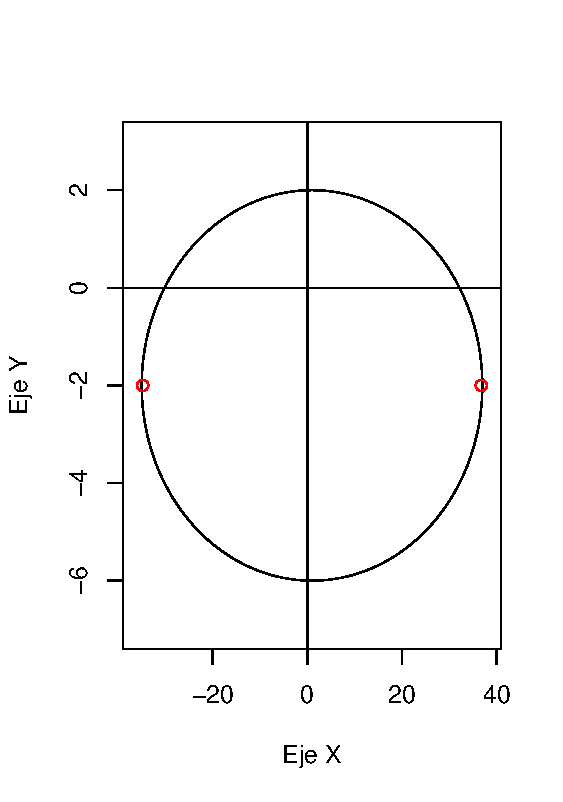
\includegraphics[scale=0.9]{Elipse2}
\caption{Gráfica de una elipse horizontal con centro en (1, -2), $a = 36$ y $b = 4$.}
\label{fig:Elipse2}
\end{figure}

\newpage
\subsection{Hipérbola}

\textbf{Definición.} Aquel lugar geometrico de un punto que se mueve en un plano de manera que el valor absoluto de la diferencia de sus distancias a dos puntos fijos en el plano, llamados $focos$ son siempre igual a una cantidad constante, positiva y menor que la distancia entre los focos.


Paa realizar esta gráfica se utilizarán  dos formas, para la grafica horizontal se tiene  primero la forma ordinaria fuera del origen: 
\begin{equation}
\frac{(x-h)^2}{a^2}-  \frac{(y-k)^2}{b^2}= 1 \label{eq:hiperbola}
\end{equation}

\citep{geometria} Despejando la variable $y$  de (\ref{eq:hiperbola})se obtiene lo siguiente:
\begin{equation}
y = k \pm \sqrt{\frac{b^2}{a^2}(x - h)^2 - b^2}, \label{eq:hiperbolahor}
\end{equation}
siendo el dominio para gráficar considerado es $x \in [h - (a + 3), h - a] \cup [h + a, h + (a + 3)]$ y para la  hipérbola vertical evaluaremos con el rango y utilizando la ecuación:
\begin{equation}
x = h \pm \sqrt{\frac{b^2}{a^2}(y - k)^2 - b^2}, \label{eq:hiperobolav}
\end{equation}
con rango de evaluación $y \in [k - (a + 3), k - a] \cup [k + a, k + (a + 3)]$.

\begin{figure}
\centering
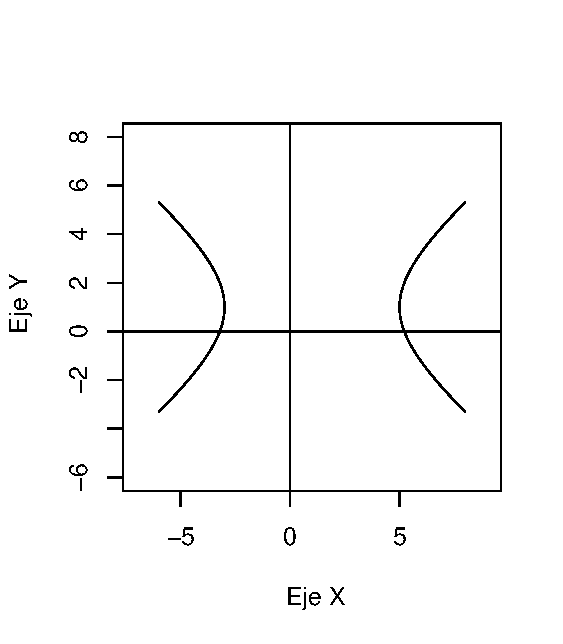
\includegraphics[scale=0.9]{Hiperbola1}
\caption{Grafica de una hipérbola sobre el eje X con centro en (1, 1), $a = 4$ y $b = 3$.}
\label{fig:Hiperbola1}
\end{figure}

\begin{figure}
\centering
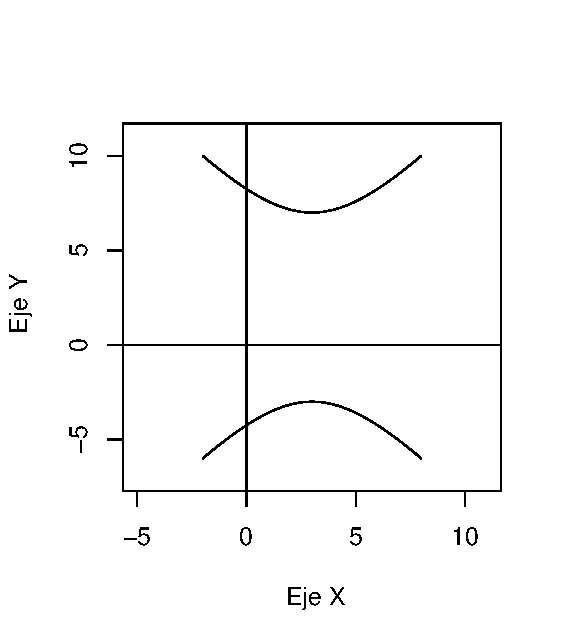
\includegraphics[scale=0.9]{Hiperbola2}
\caption{Gráfica de una hipérbola sobre el eje X con centro en (3, 2), $a = 5$ y $b = 4$.}
\label{fig:Hiperbola2}
\end{figure}

\newpage

\bibliography{bibliografia}
\bibliographystyle{plainnat}



\end{document}
